\chapter{Graph}

\section{Basic}
\rih{Graph Representation.} V for a vertex set with a map, mapping from vertex to its neighbors.
\begin{python}
V = defaultdict(list)
\end{python}

\section{BFS}
\subsection{BFS with Abstract Level}
Start BFS with a set of vertices in abstract level, not necessarily neighboring vertices.

Example:
$-1$ obstacles, $0$ targets, calculate all other vertices's Manhattan distance to its nearest target:
$$
\begin{bmatrix}
\infty & -1 & 0 & \infty \\
\infty & \infty & \infty & -1 \\
\infty & -1 & \infty & -1 \\
0 & -1 & \infty & \infty \\
\end{bmatrix} 
$$

is calculated as:
$$
\begin{bmatrix}
3 & -1 & 0 & 1 \\
2 & 2 & 1 & -1 \\
1 & -1 & 2 & -1 \\
0 & -1 & 3 & 4 \\
\end{bmatrix}
$$

\subsubsection*{Code}
\begin{python}
def wallsAndGates(self, mat):
    q = [(i, j) for i, row in enumerate(mat) 
         for j, val in enumerate(row) if val == 0]
    for i, j in q:  # iterator
        for d in self.dirs:
            I, J = i+d[0], j+d[1]
            if (0 <= I < m and  0 <= J < n and 
                mat[I][J] > mat[i][j]+1):
                mat[I][J] = mat[i][j]+1
                q.append((I, J))
\end{python}



\section{Detect Acyclic}
\begin{enumerate}
\item \pythoninline{marked} is reset after a dfs. 
\item \pythoninline{visited} should be maintained only in the end of the dfs. 
\item For directed graph:
\begin{enumerate}
\item Should dfs for all neighbors except for vertices in \pythoninline{visited}, to avoid revisiting. For example, avoid revisiting A, B when start from C in the graph $C \rightarrow A \rightarrow B$.
\item Excluding predecessor \pythoninline{pi} is erroneous in the case of $A \leftrightarrow B$ 
\end{enumerate}
\item For undirected graph:
\begin{enumerate}
\item Should dfs for all neighbors except for the predecessor \pythoninline{pi}. 
\item Excluding neighbors in \pythoninline{visited} is redundant. 
\end{enumerate}
\end{enumerate}}

\subsection{Directed Graph}

\begin{python}
def dfs(self, V, k, visited, pathset):
    if k in pathset:
        return False

    marked.add(k)
    for nbr in V[k]:
        if nbr not in visited:
            if not self.dfs(V, nbr, visited, pathset):
                return False

    marked.remove(k)
    pathset.add(k)
    return True
\end{python}
\subsection{Undirected Graph}
\begin{python}
def dfs(self, V, k, pi, visited, marked):
    if k in marked:
        return False

    marked.add(k)
    for neighbor in V[k]:
        if neighbor != pi:
            if not self.dfs(V, neighbor, k, 
                visited, marked):
                return False

    marked.remove(k)
    visited.add(k)
    return True
\end{python}

\section{Topological Sorting}
For a graph $G=\{V, E\}$, $ A \rightarrow B $, then $A$ is before $B$ in the ordered list. 
\subsection{Algorithm}
General algorithm and notice.\\
 
dfs:
\begin{enumerate}
\item \textbf{Dfs neighbors first}. If the neighbors of current node is  $\neg$visited, then dfs the neighbors
\item \textbf{Dfs current node}. After visiting all the neighbors, then visit the current node and push it to the result queue.
\item Reverse. Reverse the result queue. 
\end{enumerate}

Notice:
\begin{enumerate}
\item Need to \textbf{reverse} the result queue, since the neighbors (successors) are visited first. 
\item Need to \textbf{detect cycle}; thus the dfs need to construct result queue and detect cycle simultaneously, by using two sets: $visited$ and $marked$. 
\end{enumerate}
\begin{figure}[hbtp]
\centering
\subfloat{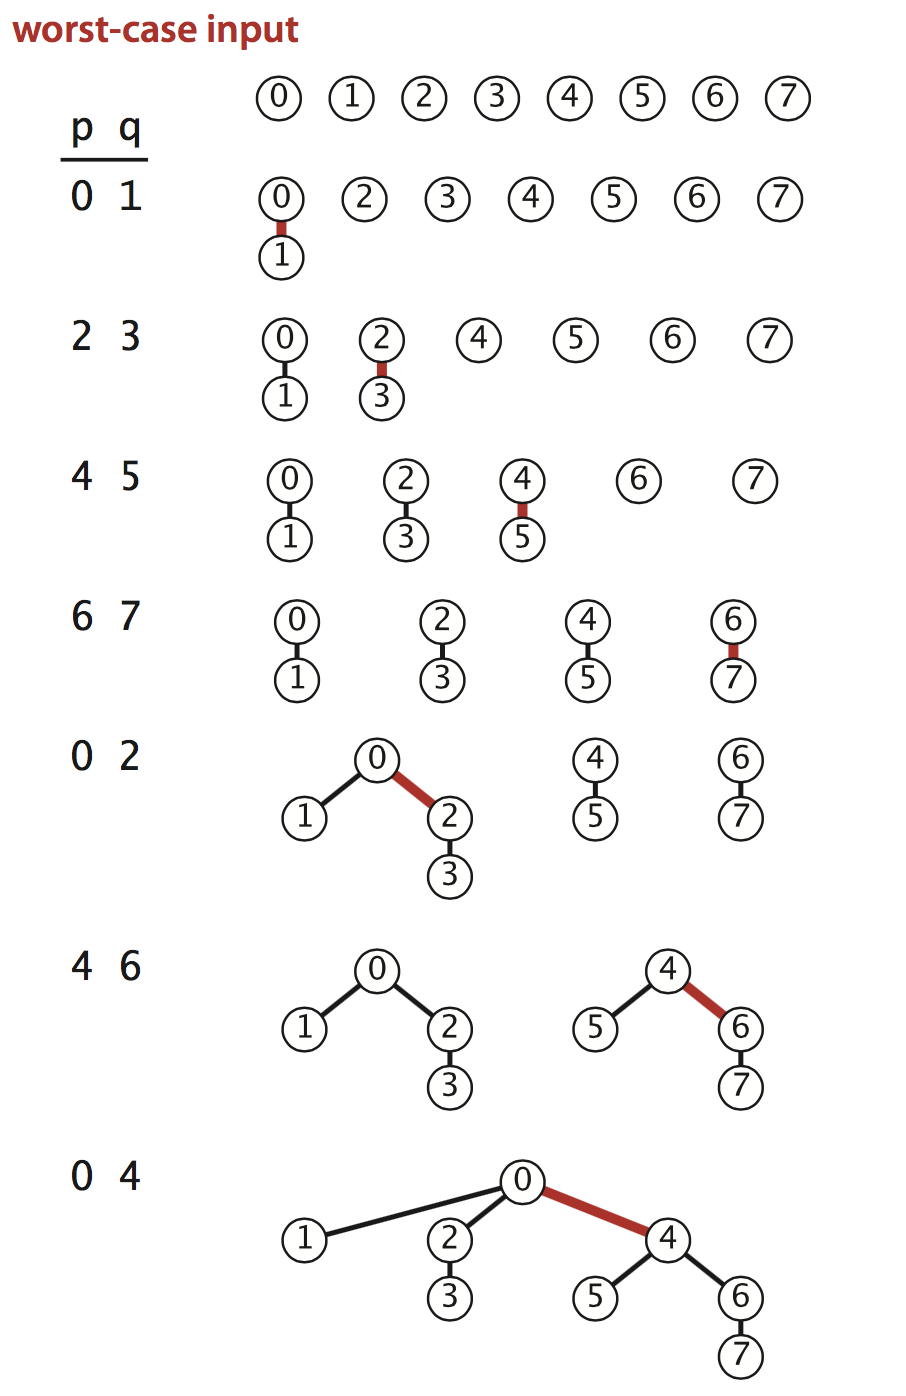
\includegraphics[scale=.60]{uf}}
\caption{Weighted quick-union traces}
\label{fig:union_find}
\end{figure}
\begin{python}
def topological_sort(self, V):
    visited = set()
    marked = set()
    ret = []

    for k in V.keys():
        if k not in visited:
            if not self.dfs(V, k, visited, marked, ret):
                return []  # contains cycle 

    ret.reverse()
    return ret

def dfs(self, V, k, visited, marked, ret):
    if k in marked:
        return False

    marked.add(k)
    for neighbor in V[k]:
        if neighbor not in visited:
            if not self.dfs(V, neighbor, visited, marked, ret):
                return False

    marked.remove(k)
    visited.add(k)
    ret.append(k)
    return True
\end{python}

\subsection{Applications}
\begin{enumerate}
\item Course scheduling problem with pre-requisite. 
\end{enumerate}

\section{Union-Find}
Improvements:
\begin{enumerate}
\item Weighting: size-baladnced tree
\item Path Compression. 
\end{enumerate}}
\subsection{Algorithm}
Weighted union-find with path compression: 
\begin{enumerate}
\item An array to store each item's predecessor \textbf{pi}. 
\item Merge the tree according to the \textbf{size} to maintain balance. 
\end{enumerate}
\begin{python}
class UnionFind(object):
    """
    Weighted Union Find with path compression
    """
    def __init__(self):
        self.pi = {}  # item -> pi
        self.sz = {}  # root -> size

    def add(self, item):
        if item not in self.pi:
            self.pi[item] = item
            self.sz[item] = 1

    def union(self, a, b):
        pi1 = self.root(a)
        pi2 = self.root(b)

        if pi1 != pi2:
            if self.sz[pi1] > self.sz[pi2]:
                pi1, pi2 = pi2, pi1
                # size balancing

            self.pi[pi1] = pi2
            self.sz[pi2] += self.sz[pi1]
            del self.sz[pi1]

    def root(self, item):
        pi = self.pi[item]
        if item != pi:
            self.pi[item] = self.root(pi)
            # path compression 

        return self.pi[item]
        
    def count(self):
        return len(self.sz)  # only root nodes have size
\end{python}

\subsection{Complexity}
$m$ union-find with $n$ objects: $O(n)+m O(\lg n)$

